\section{Introduction}

Voice interaction --- an important aspect of the life of each person. Automation of this voice interaction is developing intensively, especially in such areas as robotics \cite{Ishiguro_2016}, internet of things (IOT) and automation of many processes, in particular transport \cite{eng_Kravchenko_2009,Heisterkamp_2001} and distribution \cite{eng_art2,conf9}. The introduction of voice interfaces helps to free hands from technical device management and make this process more user-friendly and natural for a person.

Formalization of voice interaction is a rather important direction. In most systems, this is achieved by translating voice information into text with subsequent use. This approach is quite widespread and there is a large number of ready-to-use voice recognition systems in the text, but for providing high quality, such systems require a large amount of resources, so they are usually installed on servers, and their use requires permanent access to the Internet for communication with them. In addition, to use the systems of formalization of voice information in automated control systems is not enough to translate voice information into the text, it is necessary to further determine the controll influence of the received command.

There are systems of voice control that do not require voice recognition or transformation into a text form, and can immediately determine the controlling influence of the pronounced command. For example reflex voice-activated control systems \cite{eng_Egorchenkov_2016,Teslia_2014,eng_Teslia_2013}, on the basis of the theory of non-force interaction theory \cite{eng_Teslia_2010}, operate on this principle and consist of two main parts: the phonemic transcriptor \cite{eng_Pylypenko_2008}, which converts a sound recording to a phonemic representation, and a classification kernel that defines the content and control of the received phoneme set.

For automation of voice interaction, certain pre-created voice interaction scenarios \cite{eng_art3} can be used to help the system determine the meaning of what is said. Creating such interaction scenarios makes sense for technological situations in which interaction occurs under a specific protocol, for example, in industrial systems, negotiation with dispatchers in various fields: medicine, aviation \cite{eng_Korsun_2013}, law enforcement agencies or distribution \cite{eng_art3}. The creation of voice interaction scenarios for free communication is not yet so important economic value, but such attempts also exist, for example, to overcome shyness \cite{Ishiguro_2016}.

The central part of the formalization of voice interaction is the classification of spoken commands among pre-created possible scenarios of interaction. Various methods of machine learning can be used to perform this classification.

\section{The goal of the work}

The purpose of the paper is to compare the effectiveness of machine learning methods for the formalization of voice interaction on an example of a system for maintaining dispatching vehicles using a reflex voice control system.

\section{Presentation of the main material}

Reflexive voice control systems consist of two main parts: the phonemic transcriptor \cite{eng_Pylypenko_2008}, which converts the sound recording to the phonemes representation, and the classification kernel, which defines the content and control effect of each of the received phonemic sets. A dual system for the classification of the phonemic representation of voice commands \cite{eng_art4} was proposed as the classification kernel, which can use the method of intelligent reflex systems (IRS) \cite{eng_Egorchenkov_2016} or the method of convolutional neural networks (CNN) for various subject domains, depending on, which shows better results.

Convolutional neural networks for working with phonemes are most similar to the use of the  convolutional neural networks for the task of classifying texts \cite{Kim_2014}, but operate with "text" not by words, but phoneme-by-phoneme, which is similar to working with text character-by-character \cite{Zhang_2015}.

A model of voice interaction between the driver and vehicle dispatch support system was developed in the form of a scenario tree \cite{eng_art4}, which consists of 64 main commands (reactions) and divides the whole set of voice interaction into 19 contexts that can be modeled separately.

In order to test the effectiveness of the constructed models, an iterative process of data collection and modeling was conducted that included analysis of the results and the introduction of new evaluation criteria if the previous ones did not give sufficient accuracy of the assessment. In general, this process of approbation of the means of formalizing voice information in the systems of dispatch control over motor traffic can be divided into two main stages.

At the first stage, a wide data-set of voice data was gathered according to the model of the voice interaction scenarios tree in support systems for the dispatching of vehicles. The collected voice data can be described by the following parameters:

\begin{itemize}
	\item 4 devices, 23 speakers (11 women, 12 men), 94 variants of stimuli (64 on basic reactions), 3046 samples;
	\item 23 additional stimuli and 465 voice samples for the time recognition reaction.
\end{itemize}

The detailed distribution of voice data collected during the first modeling phase is presented in the table \ref{tbl:data1_distribution}. This table shows the distribution of collected voice patterns for devices and speakers, and also reports the total number of voice samples dictated by each speaker, the number of unique responses and variations of the formulation of incentives by different words among the collected voice samples. A separate column displays the number of additional records for the time recognition response.

\begin{mytable}[ht]{ | c | c | c | c | c | c | c | }%
	{Detailed distribution of speakers and voice data collected during the first stage of modeling}%
	{\label{tbl:data1_distribution}}%
	{
		\specialcell{3cm}{Speaker} & 
		\specialcell{3cm}{Device} & 
		\specialcell{3cm}{Sex} & 
		\specialcell{3cm}{Number of \\ samples} & 
		\specialcell{3cm}{Number of \\ reactions} &
		\specialcell{3cm}{Number of \\ variants of stimuli} & 
		\specialcell{3cm}{Number of samples \\ for the time \\ recognition reaction}}
	
	1 & 1 & fem. & 109 & 64 & 92 & 22 \\
	\hline
	2 & 1 & fem. & 105 & 64 & 96 & 22 \\
	\hline
	3 & 1 & fem. & 100 & 64 & 96 & 21 \\
	\hline
	4 & 1 & fem. & 97 & 64 & 93 & 22 \\
	\hline
	5 & 1 & fem. & 96 & 64 & 93 & 22 \\
	\hline
	6 & 1 & fem. & 95 & 64 & 94 & 22 \\
	\hline
	7 & 1 & fem. & 95 & 64 & 95 & 23 \\
	\hline
	8 & 1 & fem. & 95 & 62 & 90 & 21 \\
	\hline
	9 & 1 & fem. & 90 & 62 & 89 & 22 \\
	\hline
	10 & 1 & fem. & 79 & 58 & 79 & 23 \\
	\hline
	11 & 1 & masc. & 196 & 64 & 96 & 44 \\
	\hline
	12 & 1 & masc. & 101 & 64 & 94 & 25 \\
	\hline
	13 & 1 & masc. & 96 & 64 & 92 & 22 \\
	\hline
	14 & 1 & masc. & 98 & 63 & 95 & 21 \\
	\hline
	15 & 1 & masc. & 89 & 63 & 85 & 22 \\
	\hline
	16 & 1 & masc. & 98 & 62 & 90 & 21 \\
	\hline
	17 & 1 & masc. & 64 & 48 & 62 & 22 \\
	\hline
	18 & 1 & masc. & 30 & 25 & 30 & 0 \\
	\hline
	19 & 1 & masc. & 23 & 16 & 22 & 0 \\
	\hline
	20 & 1 & masc. & 23 & 9 & 19 & 0 \\
	\hline
	21 & 2 & fem. & 97 & 64 & 94 & 22 \\
	\hline
	22 & 3 & masc. & 96 & 64 & 96 & 22 \\
	\hline
	23 & 4 & masc. & 99 & 64 & 96 & 24 \\
	
\end{mytable}%

As you can see, not all speakers dictated a complete list of reactions according to the voice interaction model in dispatch support systems. This makes sense, since not all drivers will be faced with all possible unscheduled events. Also, some speakers dictated completely identical phrases several times to be able to exclude the effect of third-party noises and a certain stochastic pronunciation of and pronunciation of the sound, and some speakers dictated different variants of the formulation and pronunciation of incentives that would be able to teach the system to allocate key information in various language formulations of the natural language

The modeling by the method of intelligent reflex systems with the size of N-grams 1--3 was carried out the first. The modeling results are given in the table \ref{tbl:total_data1_irs13}. A separate model was created for each context of interaction of the driver and vehicle dispatch support system. Additional model fas created for recognition for the entire data-set, without the use of contexts. In addition to the contexts presented in the voice interaction model, an additional test context was used that consisted of three reactions of the simplest tree of scenario voice interaction \cite{eng_art3}.

\begin{mytable}[ht]{ | c | c | c | c | c | c | }%
	{The modeling results of first data-set using the method of intelligent reflex systems with the size of N-grams 1--3}%
	{\label{tbl:total_data1_irs13}}%
	{
		\specialcell{3cm}{Context \#} & 
		\specialcell{3cm}{Accuracy} & 
		\specialcell{3cm}{Average percision} & 
		\specialcell{3cm}{Average recall} & 
		\specialcell{3cm}{Average F-score} & 
		\specialcell{3cm}{Number of samples}}	
	
	1 & 0.677 & 0.450 & 0.445 & 0.447 & 124 \\
	\hline
	2 & 0.456 & 0.559 & 0.663 & 0.408 & 513 \\
	\hline
	3 & 0.387 & 0.055 & 0.143 & 0.080 & 217 \\
	\hline
	4 & 0.375 & 0.217 & 0.271 & 0.171 & 104 \\
	\hline
	5 & 0.339 & 0.108 & 0.184 & 0.111 & 183 \\
	\hline
	6 & 0.397 & 0.198 & 0.252 & 0.222 & 209 \\
	\hline
	7 & 0.206 & 0.021 & 0.098 & 0.034 & 233 \\
	\hline
	8 & 0.346 & 0.182 & 0.179 & 0.107 & 217 \\
	\hline
	9 & 0.344 & 0.144 & 0.225 & 0.141 & 131 \\
	\hline
	10 & 0.349 & 0.489 & 0.255 & 0.194 & 126 \\
	\hline
	11 & 0.268 & 0.099 & 0.145 & 0.114 & 239 \\
	\hline
	12 & 0.264 & 0.303 & 0.250 & 0.238 & 201 \\
	\hline
	13 & 0.450 & 0.361 & 0.259 & 0.182 & 171 \\
	\hline
	14 & 0.439 & 0.551 & 0.432 & 0.432 & 139 \\
	\hline
	15 & 0.302 & 0.547 & 0.210 & 0.152 & 159 \\
	\hline
	16 & 0.478 & 0.539 & 0.470 & 0.450 & 115 \\
	\hline
	17 & 0.271 & 0.261 & 0.263 & 0.248 & 155 \\
	\hline
	18 & 0.418 & 0.482 & 0.411 & 0.407 & 110 \\
	\hline
	19 & 0.471 & 0.650 & 0.458 & 0.462 & 87 \\
	\hline
	\specialcell{3cm}{Entire data-set} & 0.044 & 0.027 & 0.017 & 0.009 & 2069 \\
	\hline
	\specialcell{3cm}{Test context} & 0.485 & 0.162 & 0.333 & 0.218 & 101 \\
\end{mytable}

Dimensions of N-grams 1--3 were selected based on the fact that the method of intelligent reflex systems has a quadratic complexity of the calculation speed from the maximum size of N-gram. The table \ref{tbl:total_data1_irs13} shows that the recognition accuracy of these models does not exceed 50\% for any context other than the first one. Therefore, to improve the quality of the models, simulation was carried out using the same method, but with the size of N-grams 2--4. The results of this simulation are presented in the table \ref{tbl:total_data1_irs24}.


\begin{mytable}[ht]{ | c | c | c | c | c | c | }%
	{The modeling results of first data-set using the method of intelligent reflex systems with the size of N-grams 2--4}%
	{\label{tbl:total_data1_irs24}}%
	{
		\specialcell{3cm}{Context \#} & 
		\specialcell{3cm}{Accuracy} & 
		\specialcell{3cm}{Average percision} & 
		\specialcell{3cm}{Average recall} & 
		\specialcell{3cm}{Average F-score} & 
		\specialcell{3cm}{Number of samples}}		
	
	1 & 0.710 & 0.503 & 0.442 & 0.459 & 124 \\
	\hline
	2 & 0.895 & 0.465 & 0.478 & 0.471 & 513 \\
	\hline
	3 & 0.382 & 0.048 & 0.124 & 0.069 & 217 \\
	\hline
	4 & 0.558 & 0.740 & 0.480 & 0.484 & 104 \\
	\hline
	5 & 0.415 & 0.434 & 0.259 & 0.225 & 183 \\
	\hline
	6 & 0.565 & 0.282 & 0.359 & 0.316 & 209 \\
	\hline
	7 & 0.232 & 0.388 & 0.127 & 0.089 & 233 \\
	\hline
	8 & 0.373 & 0.410 & 0.207 & 0.157 & 217 \\
	\hline
	9 & 0.527 & 0.737 & 0.437 & 0.449 & 131 \\
	\hline
	10 & 0.532 & 0.773 & 0.468 & 0.486 & 126 \\
	\hline
	11 & 0.515 & 0.207 & 0.282 & 0.238 & 239 \\
	\hline
	12 & 0.488 & 0.510 & 0.469 & 0.452 & 201 \\
	\hline
	13 & 0.485 & 0.448 & 0.303 & 0.283 & 171 \\
	\hline
	14 & 0.633 & 0.703 & 0.625 & 0.625 & 139 \\
	\hline
	15 & 0.453 & 0.480 & 0.329 & 0.333 & 159 \\
	\hline
	16 & 0.583 & 0.661 & 0.574 & 0.550 & 115 \\
	\hline
	17 & 0.387 & 0.473 & 0.378 & 0.374 & 155 \\
	\hline
	18 & 0.582 & 0.672 & 0.576 & 0.583 & 110 \\
	\hline
	19 & 0.655 & 0.728 & 0.650 & 0.642 & 87 \\
	\hline
	\specialcell{3cm}{Entire data-set} & 0.122 & 0.061 & 0.048 & 0.027 & 2069 \\
	\hline
	\specialcell{3cm}{Test context} & 0.475 & 0.160 & 0.327 & 0.215 & 101 \\
\end{mytable}

As an alternative classifier in the dual system of classification of phonemic representation of voice commands, the method of convolutional neural networks \cite{eng_art4} was used. Unlike the method of intelligent reflex systems, the method of convolutional neural networks depends on the size of the filters only linearly, because instead of all possible N-grams, only a certain fixed number of filters that are learned by the method of error propagation are used. Therefore, only filter sizes 2--4 were used to model convolutional neural networks. The results of this simulation are presented in the table \ref{tbl:total_data1_cnn}.

\begin{mytable}[ht]{ | c | c | c | c | c | c | }%
	{The modeling results of first data-set using the method of convolutional neural networks with the size of N-grams 2--4}%
	{\label{tbl:total_data1_cnn}}%
	{
		\specialcell{3cm}{Context \#} & 
		\specialcell{3cm}{Accuracy} & 
		\specialcell{3cm}{Average percision} & 
		\specialcell{3cm}{Average recall} & 
		\specialcell{3cm}{Average F-score} & 
		\specialcell{3cm}{Number of samples}}	
	
	1 & 0.879 & 0.880 & 0.863 & 0.870 & 124 \\
	\hline
	2 & 0.957 & 0.933 & 0.799 & 0.851 & 513 \\
	\hline
	3 & 0.820 & 0.870 & 0.777 & 0.813 & 217 \\
	\hline
	4 & 0.846 & 0.857 & 0.829 & 0.837 & 104 \\
	\hline
	5 & 0.798 & 0.814 & 0.734 & 0.754 & 183 \\
	\hline
	6 & 0.852 & 0.851 & 0.789 & 0.814 & 209 \\
	\hline
	7 & 0.785 & 0.808 & 0.773 & 0.785 & 233 \\
	\hline
	8 & 0.871 & 0.895 & 0.847 & 0.867 & 217 \\
	\hline
	9 & 0.863 & 0.871 & 0.836 & 0.847 & 131 \\
	\hline
	10 & 0.825 & 0.841 & 0.818 & 0.819 & 126 \\
	\hline
	11 & 0.908 & 0.922 & 0.850 & 0.878 & 239 \\
	\hline
	12 & 0.846 & 0.852 & 0.849 & 0.847 & 201 \\
	\hline
	13 & 0.848 & 0.860 & 0.842 & 0.849 & 171 \\
	\hline
	14 & 0.842 & 0.851 & 0.838 & 0.838 & 139 \\
	\hline
	15 & 0.849 & 0.842 & 0.829 & 0.834 & 159 \\
	\hline
	16 & 0.817 & 0.826 & 0.814 & 0.814 & 115 \\
	\hline
	17 & 0.723 & 0.729 & 0.723 & 0.720 & 155 \\
	\hline
	18 & 0.836 & 0.842 & 0.837 & 0.835 & 110 \\
	\hline
	19 & 0.862 & 0.871 & 0.863 & 0.856 & 87 \\
	\hline
	\specialcell{3cm}{Entire data-set} & 0.652 & 0.679 & 0.622 & 0.640 & 2069 \\
	\hline
	\specialcell{3cm}{Test context} & 0.891 & 0.915 & 0.871 & 0.888 & 101 \\
\end{mytable}

The tables \ref{tbl:total_data1_irs13}, \ref{tbl:total_data1_irs24} and \ref{tbl:total_data1_cnn} include some measurements of model quality and the number of samples used to study and evaluate models. First, the accuracy \cite{Ting_2011} was used as the main measure, which can be calculated using the following formula:

\begin{equation}
\label{eq:acuracy}
A=\frac{\sum\limits_i TP_i}{\sum\limits_i TP_i+FN_i},
\end{equation}

where $A$ is the accuracy, $TP_i$ is the number of true positive samples of the reaction $i$, a $FN_i$ is the number of false negative samples of the reaction $i$.

Since the frequency of reactions in most contexts is not balanced, accuracy may show better results than the true quality of the model.

By constructing graphs of accuracy distribution and F-score from the number of samples in a context (Fig. \ref{img:accuracy_distribution_data1}) we can see that there is no direct dependence. But the quality of recognition should be influenced by the number of reactions in the context and the average number of records of samples of voice data for each reaction.

\begin{figure}[!t]
	\centering
	\subbottom[The IRS method with 1--3 N-gram sizes \label{img:accuracy_distribution_data1_irs13}]{%
		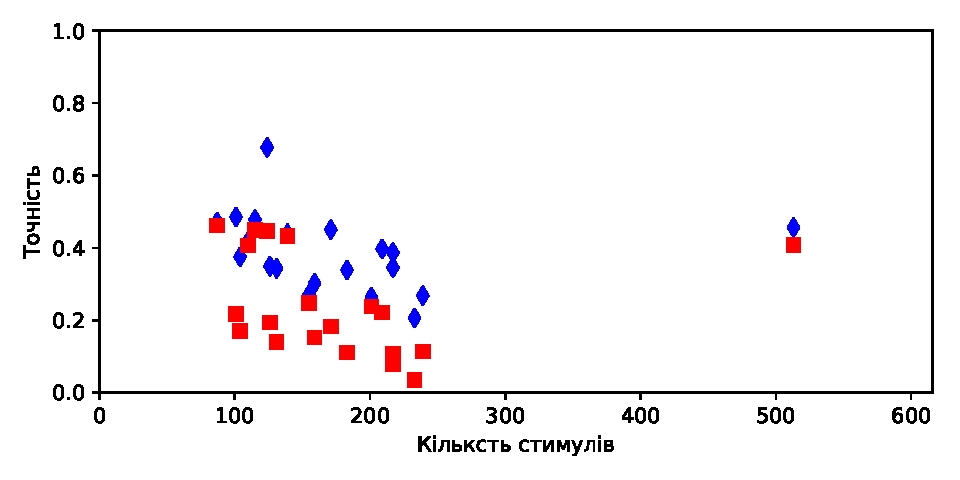
\includegraphics[width=.7\linewidth]{accuracy_distribution_data1_irs13}}
	\\
	\subbottom[The IRS method with 2--4 N-gram sizes \label{img:accuracy_distribution_data1_irs24}]{%
		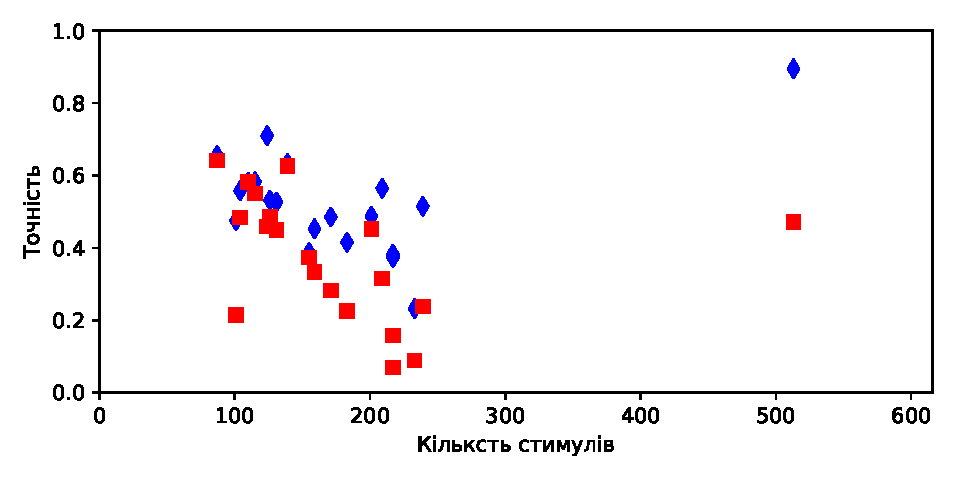
\includegraphics[width=.7\linewidth]{accuracy_distribution_data1_irs24}}
	\\
	\subbottom[The CNN method with 2--4 N-gram sizes \label{img:accuracy_distribution_data1_cnn}]{%
		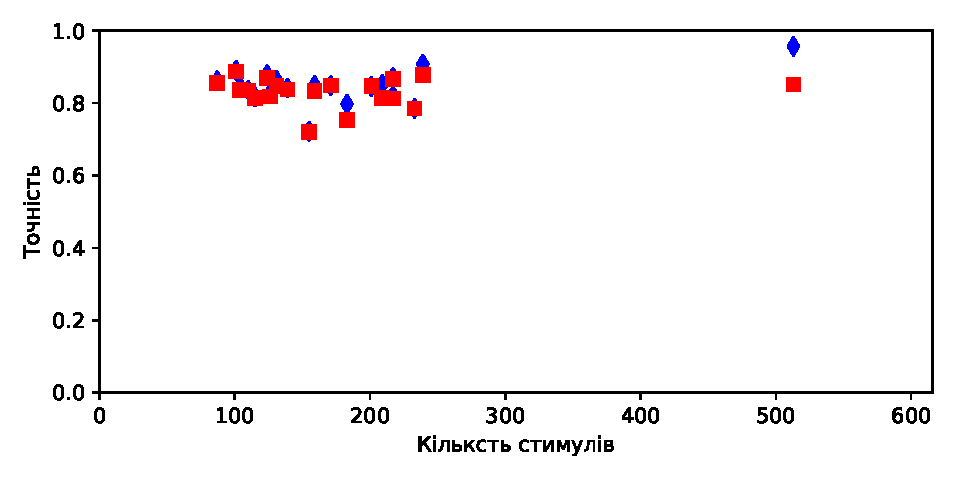
\includegraphics[width=.7\linewidth]{accuracy_distribution_data1_cnn}}
	\caption{Distribution of accuracy (red squares) and F-scoe (blue diamonds) by the number of vocal samples using different methods for modeling contexts}
	\label{img:accuracy_distribution_data1}
\end{figure}

From the confusion matrix \cite{Stehman_1997} of the modeling of the test context by the method of intelligent reflex systems (Fig. \ref{img:confusion_matrix_data1_irs13_context_21} and \ref{img:confusion_matrix_data1_irs24_context_21}), we can see that the recognition level close to 50\% is achieved due to the fact that all reactions in the context are recognized as reaction \#2. Since it is represented by the largest number of samples, the accuracy reaches relatively high values with the actual low quality of the model.

\begin{figure}[!t]
	\centering
	\subbottom[The IRS method with 1--3 N-gram sizes \label{img:confusion_matrix_data1_irs13_context_21}]{%
		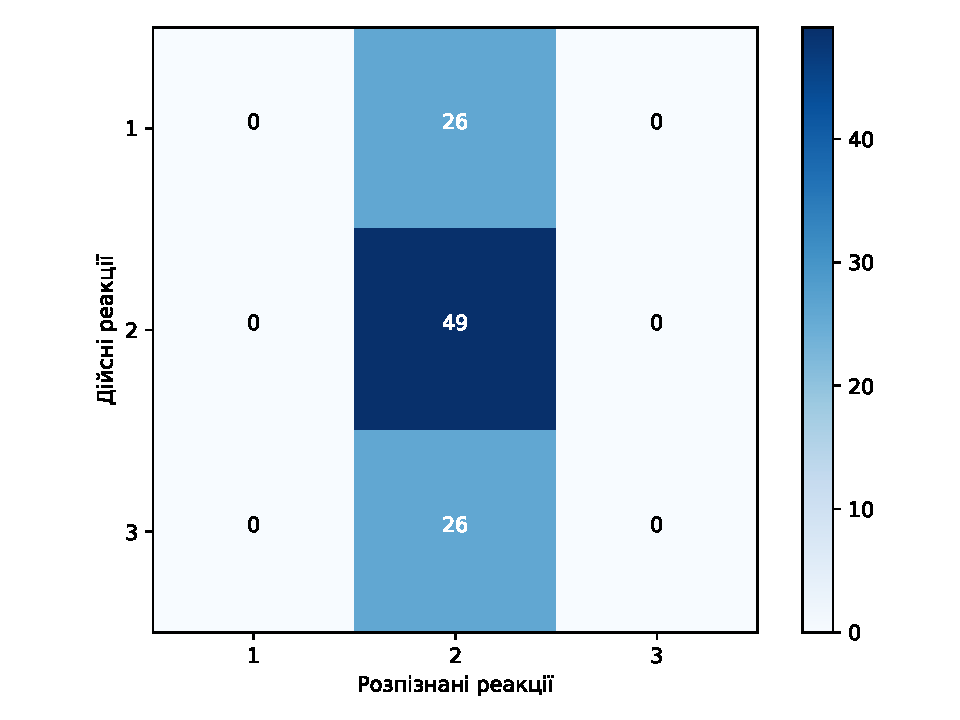
\includegraphics[width=.3\linewidth]{confusion_matrix_data1_irs13_context_21}}
	\subbottom[The IRS method with 2--4 N-gram sizes \label{img:confusion_matrix_data1_irs24_context_21}]{%
		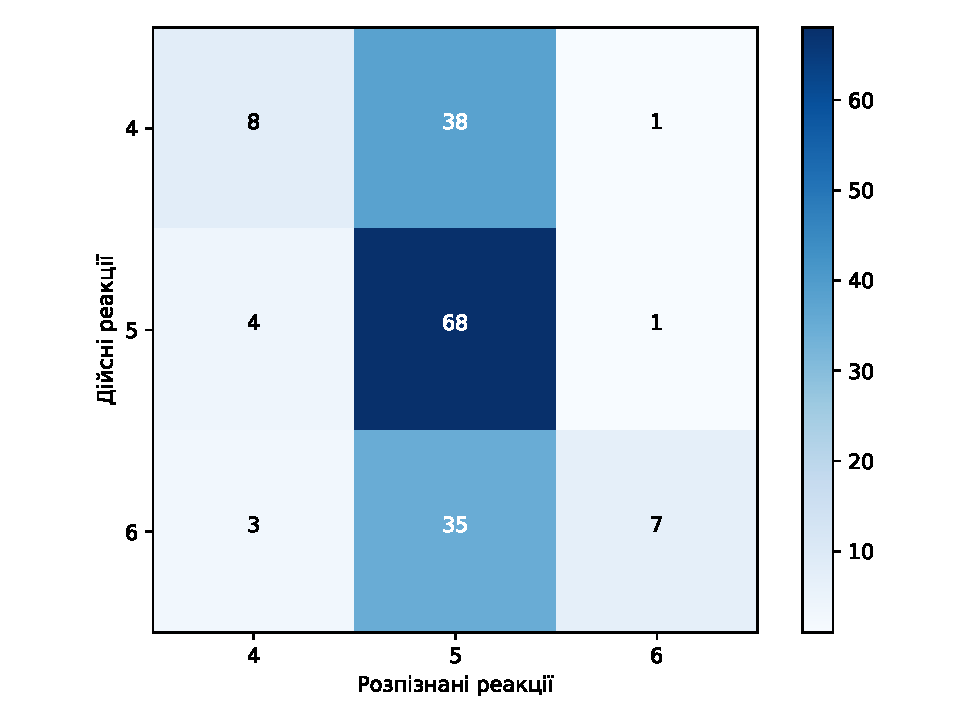
\includegraphics[width=.3\linewidth]{confusion_matrix_data1_irs24_context_13}}
	\subbottom[The CNN method with 2--4 N-gram sizes \label{img:confusion_matrix_data1_cnn_context_21}]{%
		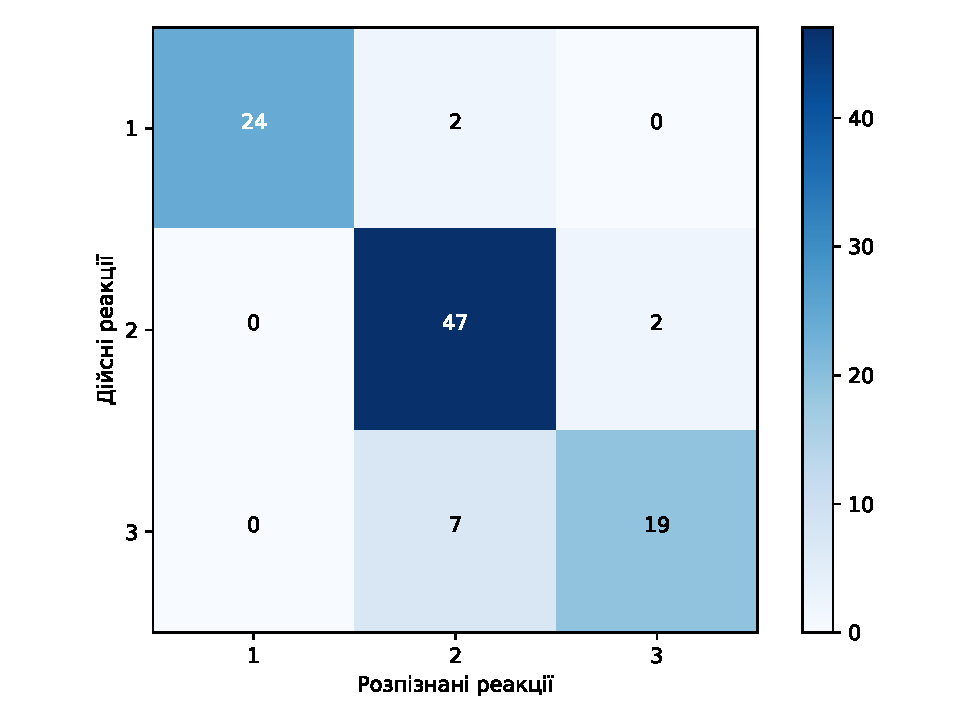
\includegraphics[width=.3\linewidth]{confusion_matrix_data1_cnn_context_21}}
	
	\caption{Comparison of confusion matrices of three different methods (a, b, c) of recognition by reactions for the test context of the first data-set}
	\label{img:confusion_matrix_data1_context_21}
\end{figure}

Having examined the confusion matrices of models of other contexts by the method of intelligent reflex systems, it was discovered that models of all contexts are more or less subject to such errors. Models of contexts 14, 16, 18 and 19 turned out to be less inclined, but according to the table, we can see that the accuracy values for these contexts are less than the accuracy of the models for the 13th and the test contexts, where all the reactions were identified as the same ( Fig. \ref{img:confusion_matrix_data1_irs13_context_21}).

As better measures of the classification model quality for unbalanced samples, precision and recall are usually used, which in the case of non-binary classification can be determined only for a particular class, and not for the model as a whole \cite{Powers_2011}. To assess the quality of the model, we used average indicators of precision and recall for all reactions that can be determined by the formulas:

\begin{equation}
\label{eq:рrecision}
P=\frac{1}{n}\sum\limits_i\frac{TP_i}{TP_i+FP_i};
\end{equation}

\begin{equation}
\label{eq:recall}
R=\frac{1}{n}\sum\limits_i\frac{TP_i}{TP_i+FN_i},
\end{equation}

where $P$ is the average precision, $R$ is the average recall, $n$ is the number of classes, $TP_i$ is the number of true positive samples of the reaction $i$, $FP_i$ --- the number of false positive samples of the reaction $i$, and $FN_i$ is the number of false negative samples of the reaction $i$.

Since the precision only shows errors of the first kind, and the recall of only errors of the second kind, there is a generalized F-score (F1, F-measure) \cite{Powers_2011, Sasaki_2007}, which takes both types of errors into account as average harmonic, and can be determined by formula:

\begin{equation}
\label{eq:f1}
F_1 = 2 \cdot \frac{P \cdot R}{P + R},
\end{equation}

where $F_1$ --- F-score, $P$ --- precision а $R$ --- recall.

Having examined the values of the F-score from the table \ref{tbl:total_data1_irs13}, we can see that the models of contexts 14, 16, 18 and 19, which look best on the error matrices, have one of the largest values of the F-score, and are compared with the values of the models of contexts 1 and 2, that consists of only two reactions. The modeling using the N-grams sizes 2-4 (tab. \ref{tbl:total_data1_irs24}) showed similar results and gave a small increase in the quality of recognition, but this quality is still not enough for the practical application of the model.

The method of convolutional neural networks showed a better result. The table \ref{tbl:total_data1_cnn} shows that the values of F-score are relativel not much lower than precision, which suggests that this model works better with unbalanced classes.

To calculate the metrics in the tables \ref{tbl:total_data1_irs13} - \ref{tbl:total_data1_cnn}, the cross-validation method \cite{Kohavi_1995} was used, splitting the complete data-set into 5 equal random parts. Thus, the modeling was carried out 5 times, so that each of the 5 parts was once used as a test set, and 4 other parts in each simulation were a training set. A combination of results on a test set of 5 partial models and was used to calculate the metrics in the tables.

The calculation of the metrics on the test set showed the accuracy of the recognition from 90\% to 100\%, indicating the effect of overfitting. One way to overcome the problem of overfitting is to increase the amount of data. The hypothesis of low recognition quality due to insufficient number of input data was put forward.

Therefore, it was decided to conduct a second phase of the study, for which it was necessary to collect more voice data. To verify the hypothesis it is decided to collect vocal samples for only one test context.

Additional voice data is collected for one context: 1 device, 1 speaker (male), 37 stimulus variants, 3 reactions in the context, 938 samples.

The results of modeling the second set of data by three different methods can be seen in the table \ref{tbl:total_data2_irs13}, and the error matrix is shown in the figure \ref{img:confusion_matrix_data2_context_21}.

\begin{mytable}{ | c | c | c | c | }%
	{Comparison of recognition quality of the second data-set by different methods}%
	{\label{tbl:total_data2_irs13}}%
	{ Measure & IRS 1--3 & IRS 2--4 & CNN }		
	
	Accuracy & 0.258 & 0.598 & 0.935 \\
	\hline
	Average precision & 0.226 & 0.636 & 0.939 \\
	\hline
	Average recall & 0.238 & 0.579 & 0.935 \\
	\hline
	Average F-score & 0.217 & 0.583 & 0.937 \\
	\hline
	Number of samples & 925 & 925 & 925 \\
\end{mytable}

\begin{figure}[ht!]
	\centering
	\subbottom[The IRS method with 1--3 N-gram sizes \label{img:confusion_matrix_data2_irs13_context_21}]{%
		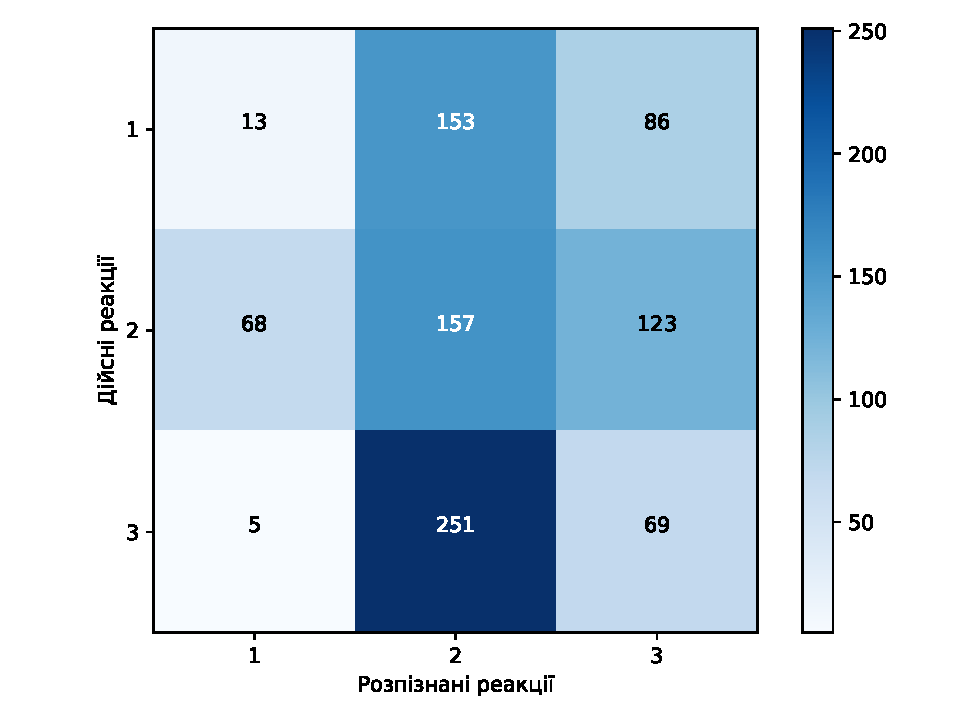
\includegraphics[width=.3\linewidth]{confusion_matrix_data2_irs13_context_21}}
	\subbottom[The IRS method with 2--4 N-gram sizes \label{img:confusion_matrix_data2_irs24_context_21}]{%
		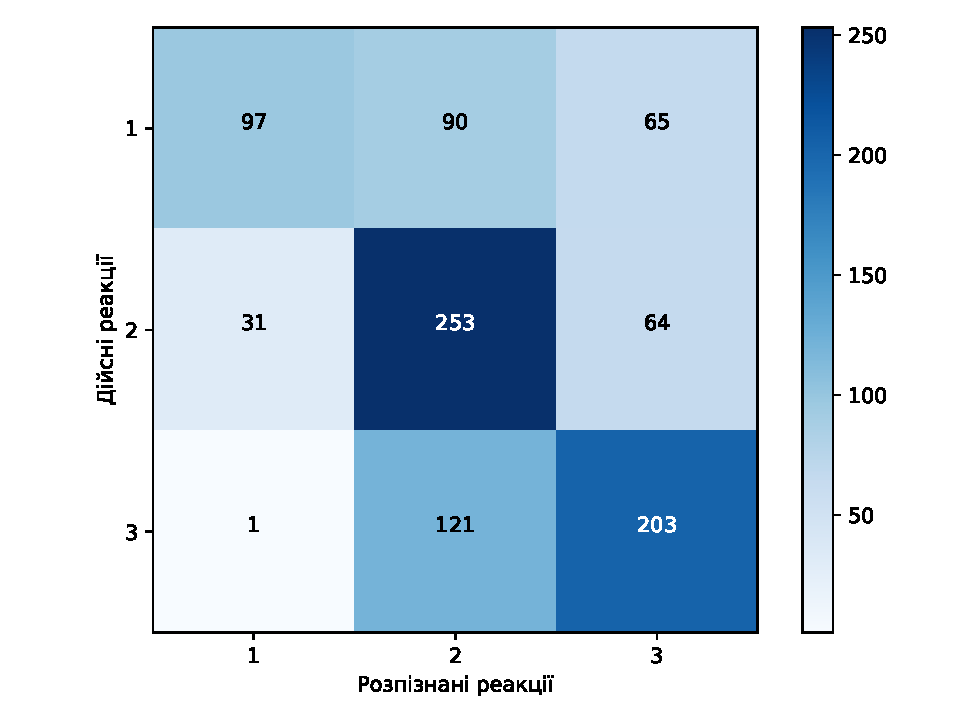
\includegraphics[width=.3\linewidth]{confusion_matrix_data2_irs24_context_21}}
	\subbottom[The CNN method with 2--4 N-gram sizes \label{img:confusion_matrix_data2_cnn_context_21}]{%
		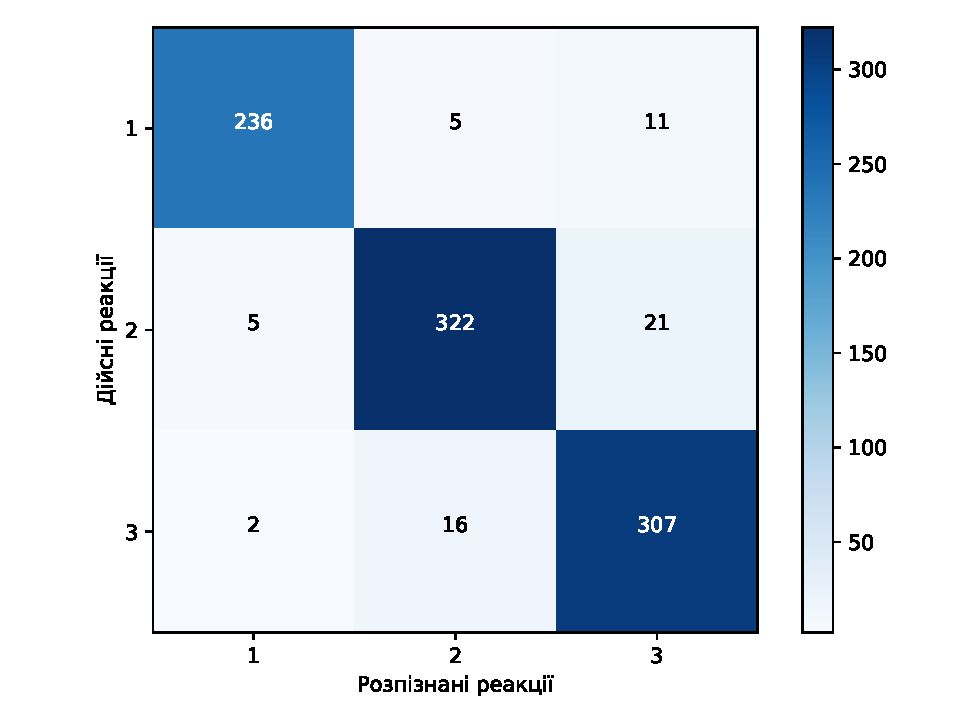
\includegraphics[width=.3\linewidth]{confusion_matrix_data2_cnn_context_21}}
	
	\caption{Comparison of confusion matrices of three different methods (a, b, c) of recognition by reactions for the test context of the second data-set}
	\label{img:confusion_matrix_data2_context_21}
\end{figure}

From the simulation results, it can be seen that an increase in the number of input data has undoubtedly improved the quality of recognition for all methods. Modeling intelligent reflex systems for one context with a large sample of data gave almost 60\% accuracy and a F-score of 0.58. The error matrix (fig. \ref{img:confusion_matrix_data2_irs24_context_21}) does not have a clear predominance of a certain reaction over others. Unfortunately, the obtained accuracy values are still not enough to successfully use the model in practice.

The modeling by convolutional neural networks gave slightly more than 90\% accuracy and the corresponding value of the F-score. Such accuracy is sufficient for practical application, so we can conclude that under these conditions the dual system of classification of the phonemic representation of voice commands works better using the method of convolutional neural networks for constructing a model of formalization of voice information in dispatching systems of motor vehicles.

\section{Discussion}

Comparison of different metrics of efficiency of models of non-binary classification has shown that for high-quality models, as well as in cases of balanced data samples, all metrics show similar efficiency values. But in cases of models that respond negatively to the imbalance of the sample, the F-measure estimates the model much more accurately.

There were 2 stages of modeling. At the initial stage, the voice data of 23 speakers was collected, with an average of 45 samples per reaction. The results of simulation by both methods showed an accuracy of not more than 50\%, which is insufficient for practical application. The accuracy of the classification in the training data was close to 100\%, indicating a overfitting.

On the basis of this, the hypothesis of insufficient number of voice data was put forward, therefore, in the second stage, an average of 310 voice samples were collected for each of the three simple context responses. The modeling by the method of intelligent reflex systems showed an accuracy of about 60\%, which is also insufficient, and the method of convolutional neural networks is slightly more than 90\%, which is acceptable.

From this it can be seen that under the given conditions, the efficiency of the method of convolutional neural networks is higher than the method of intelligent reflex systems by more than 30\%. These results are somewhat surprising, because in previous studies \cite{eng_Egorchenkov_2016,Teslia_2014,eng_Teslia_2013} the method of intelligent reflex systems gave much better results. Visually exploring the phonemic representation of data, we noticed a high noise level of phonemic data, although in sound files the noise level was lower. One possible explanation for this is that the phonemic transcript was not configured to use a microphone in a mobile phone, which frequency indicators may interfere with the system.

That is, the following hypothesis has been put forward on the lack of sound recording quality and the high level of noise as an obstacle to the effectiveness of the formalization model. The prospect of further development is the next phase of the study, for which it is necessary to collect a new sample of data using a better external microphone. In addition, in order to eliminate the effect of an unbalanced sample of data, it is proposed to collect an equal number of records for each reaction from the tree of scenario voice interaction.

\section{Conclusions}

Testing the simulation of the recognition of commands based on the iterative process of data collection and the introduction of new evaluation criteria, if the previous ones did not give sufficient accuracy of evaluation, can provide a process for comparing the effectiveness of different classification methods in the dual model of voice interaction formalization.

It is advisable to use a set of metrics for assessing the effectiveness of classification models, which must include, in addition to estimating the accuracy, the robust metrics for the unbalanced sample (such as precision, recall, F-score) or visual analysis of error matrices.

The acceptable level of accuracy for practical use in the model constructed by the method of convolutional neural networks during the second iteration of the simulation with sufficient amount of training data has been achieved.

In order to confirm the efficiency of the method of intelligent reflex systems of two iterations it was not enough, the hypothesis about insufficient quality of sound recordings and high level of noise as obstacles to the effectiveness of the formalization model was advanced, prospects for conducting the next stage of research were outlined.

In general, according to the results of the work, the efficiency of the reflex voice control system, which consists of a phonemic transcriptor and a classification kernel, is confirmed, and in practice it is possible to determine the content and control effect of the received phonemic set without converting the voice information into a text form.


